\section{Housing Dynamics and Business Cycle in the US Economy}\label{sec:Stylized_Facts}

Among aggregate demand expenditures, non-residential investment is one of the most examined (at least) between heterodox macroeconomists.
As a consequence, the relevance of other (autonomous) expenditures on macroeconomic dynamics has been underestimated (\cite{brochier_macroeconomics_2017}).
Residential investment, on the other hand, is not as studied by the literature despite being one of the most volatile expenditure (see Figure \ref{FigVolatilidade}).
Moreover, however small its share on GDP is (see Figure \ref{FigAutonomos}), it does not imply that it has negligible effects on the business cycle.
In this section, we argue that this little attention that residential investment receives is not compatible with its relevance for the US.
Furthermore, we show that this significance is not restricted to the recent housing crisis.

\begin{figure}
	\caption{Housing's Particular Stylized Facts}
	\label{fig:figs}
	\begin{subfigure}[t]{.5\textwidth}
		\centering
		\caption{Selected growth rate distribution (1947-2019)}
		\label{FigVolatilidade}
		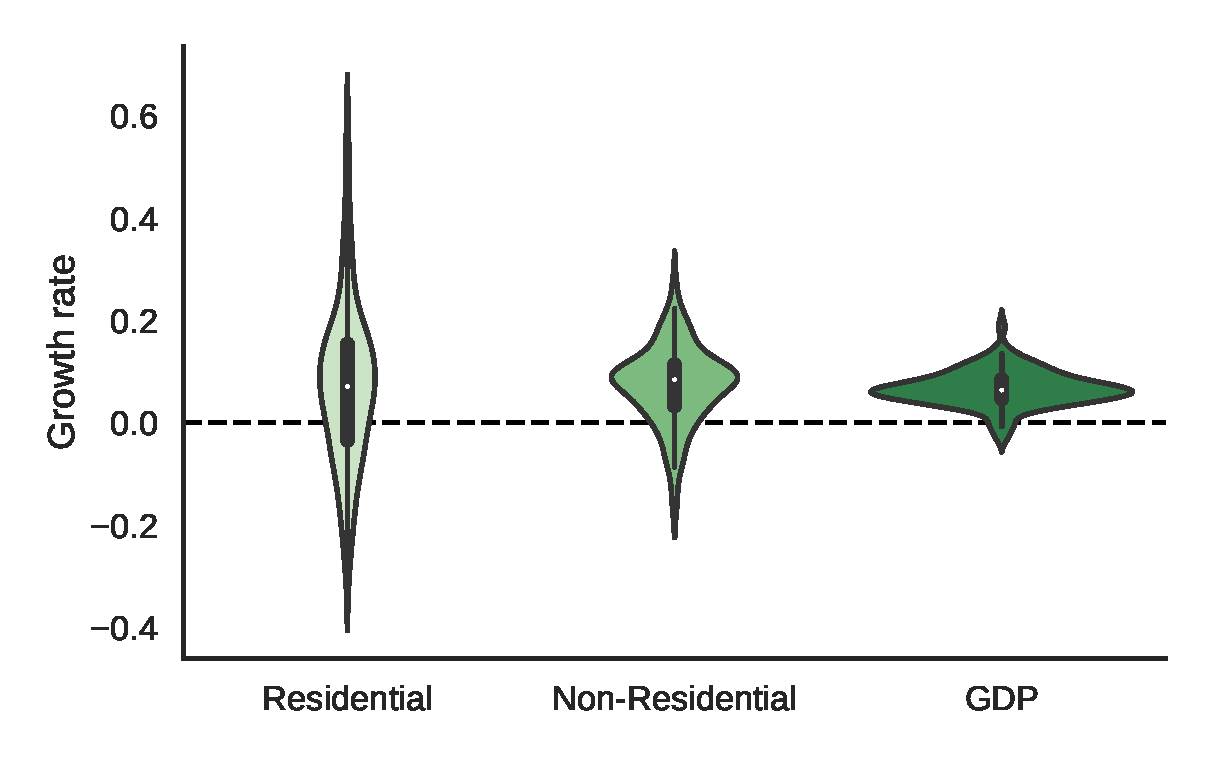
\includegraphics[width=.8\linewidth]{./figs/Volatilidade.eps}
	\end{subfigure}
	\begin{subfigure}[t]{.5\textwidth}
		\centering
		\caption{Autonomous expenditures share on GDP (US, 1979-2019)}
		\label{FigAutonomos}
		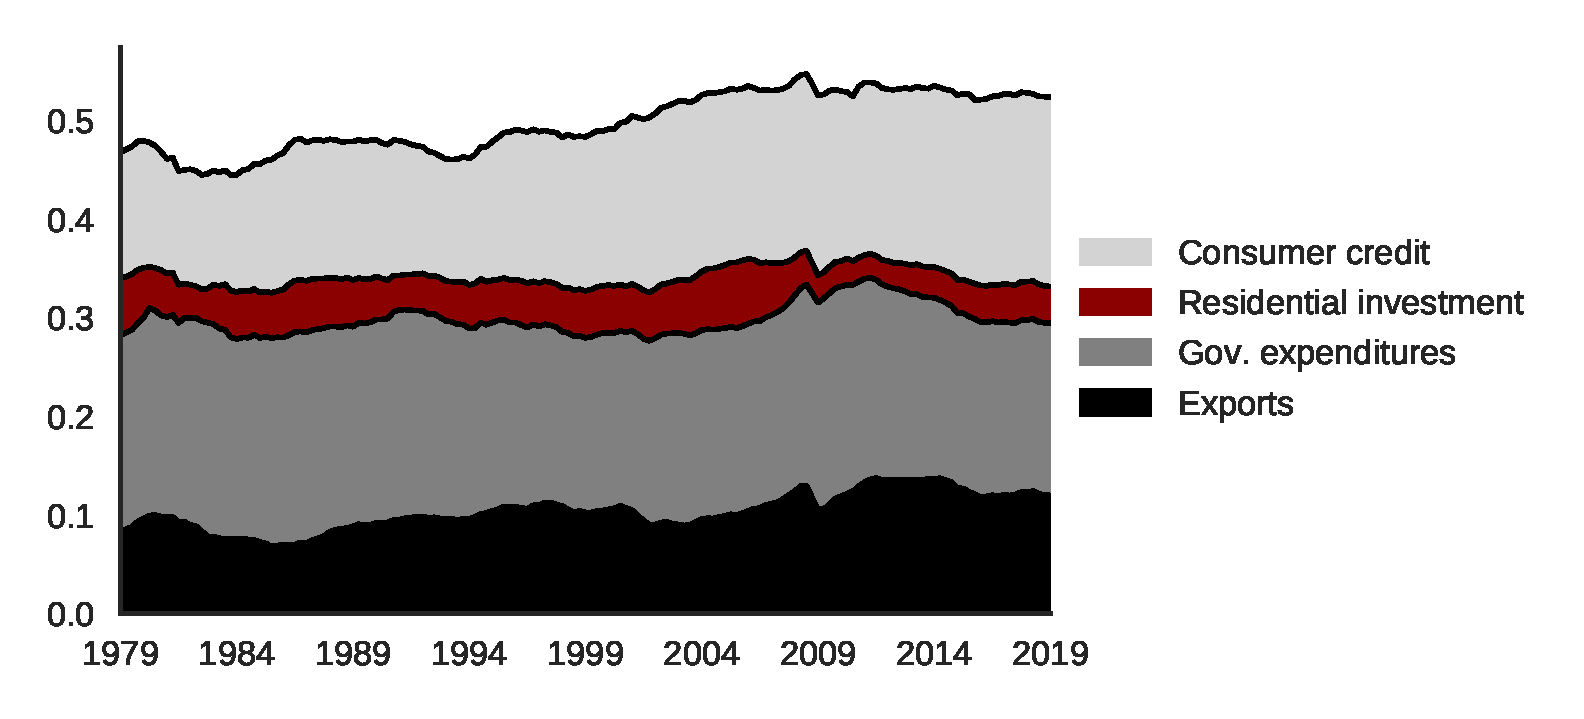
\includegraphics[width=.8\linewidth]{./figs/Gastos_autonomos.eps}  
	\end{subfigure}
	\caption*{\textbf{Source:} U.S. Bureau of Economic Analysis, Authors' Elaboration}
\end{figure}


It is worth mentioning the novelty of \textcite{green_follow_1997} and \textcite{leamer_housing_2007} --- revisited in \textcite{leamer_housing_2015} and by \textcite{fiebiger_trend_2017} --- when shedding light on the relevance of residential investment even before of the Great Recession.
More precisely, \textcite{green_follow_1997} reports that residential investment leads --- more than firms' investment --- the business cycle.
However, argues that this result does not imply a causal relationship:

\begin{quotation}
	[P]erhaps residential investment, like stock prices and interest rates, is a good predictor of GDP because it is a series that reflects \textbf{forward-looking behavior}. Presumably households will not increase their expenditures on housing unless they expect to prosper in the future. Building a house is a natural mechanism for doing this. Thus, the series can do a good job of predicting GDP \textbf{without necessarily causing GDP} (\cite[p.~267, ephasis added]{green_follow_1997}).
\end{quotation}
Despite paying attention to non-capacity creating autonomous expenditure, \textcite{green_follow_1997}, restricts its relevance as temporal precedence indicator.
\textcite{leamer_housing_2007}, on the other hand, reports a causal relationship between housing and GDP.
In summary, states that residential investment implies a higher durable goods consumption, that is, the US business cycle is a ``consumer cycle''.

Next, we present Figure \ref{FigIh_u} in order to depict the relation between housing and business cycle in which each cycle is represented in a different panel\footnote{FIEBIGER}. 
The vertical axis represents residential investment-GDP ratio and the horizontal
axis represents the rate of capacity utilization as a proxy for business cycle.
Economic recovery is generally characterized residential investment growing faster than GDP --- with the 1991-2000 period being a particular case. 
As a consequence of this higher growth rate, is the increase of both residential investment share on GDP and capacity utilization. 
Following the Sraffian supermultiplier growth model, we conclude that increase of non-residential investment is the result of capital stock adjustment principle.
This increase implies GDP to grow faster than residential investment, therefore reducing both its share on GDP and capacity utilization ratio. 
Finally, as a result of economic burst, capacity utilization ratio falls and the cycle.


\begin{figure}[H]
	\centering
	\caption{Residential investment share on GDP VS. capacity utilization during recessions}
	\label{FigIh_u}
	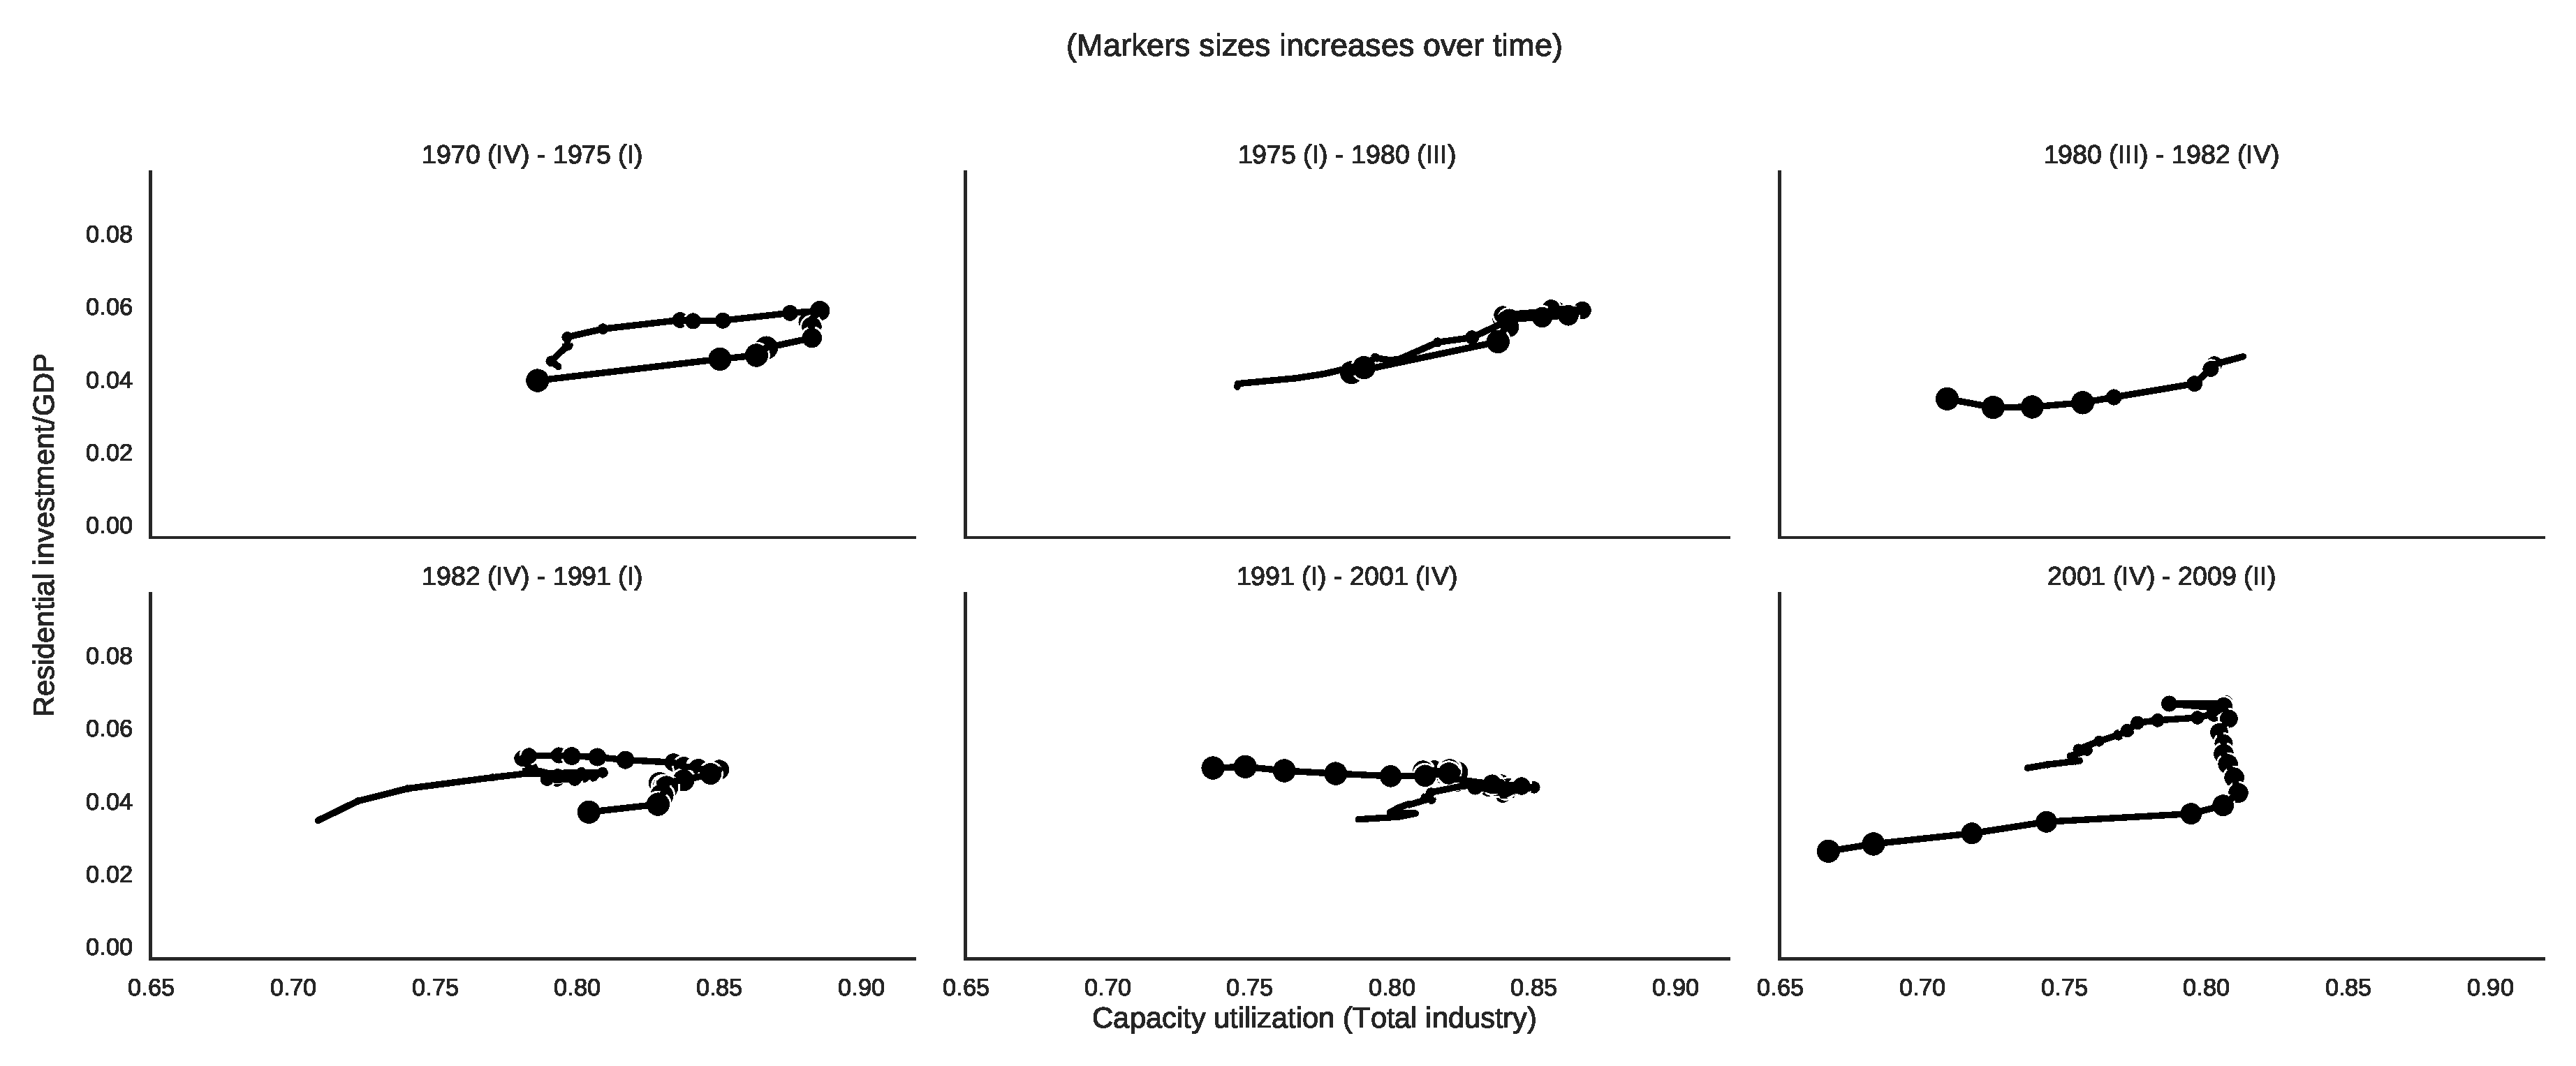
\includegraphics[width=\textwidth]{./figs/Ciclo_Ih_u.eps}
	\caption*{\textbf{Source:} Authors' Elaboration}
\end{figure}

There is also an indirect relation between housing and aggregate demand. 
Real estate constitutes a significant portion of household wealth so houses serves as collateral to borrowing (\cite{teixeira_uma_2011}). 
As a consequence of US institutional arrangement, households --- especially the poorest ones --- could increase their indebtedness as houses prices went up (see Figure \ref{FigDividaPreco}) as a way to ``realize'' capital gains without
selling their homes during house bubble of the 2000s (\cite{teixeira_crescimento_2015}).
Therefore, real estate inflation and durable goods consumption are connected and has relevant consequences for business cycle.
\textcite{zezza_u.s._2008} and \textcite{barba_rising_2009}, for example, report that credit-financed consumption was one of the main drivers of economic growth before the Great Recession.




\begin{figure}[H]
	\centering
	\caption{Household indebtedness and house prices dynamics (jan/2000=100)}
	\label{FigDividaPreco}
	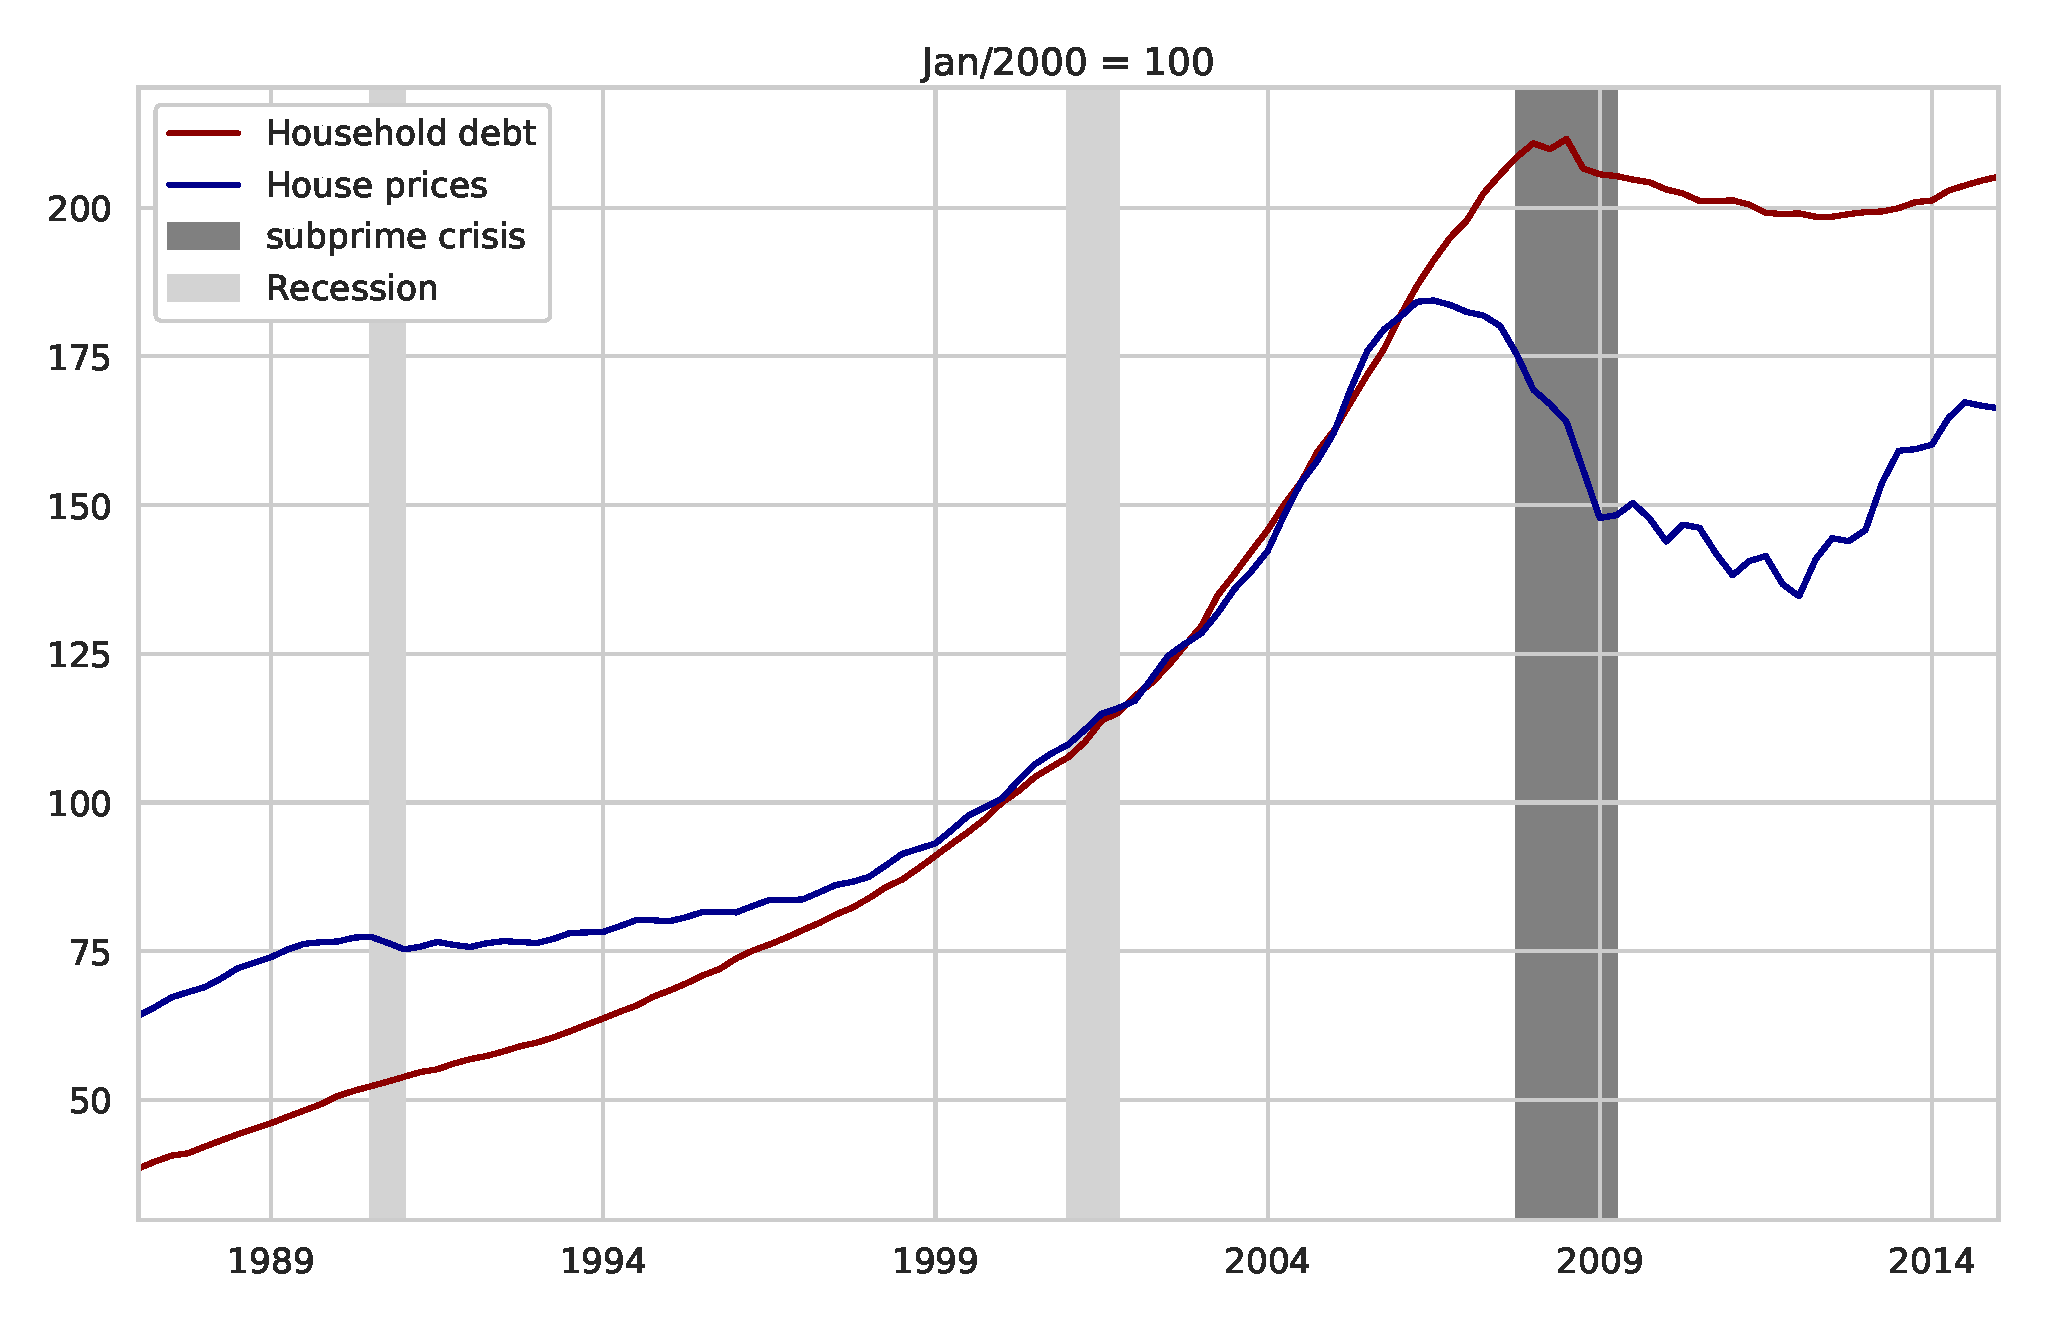
\includegraphics[width=\textwidth]{./figs/Divida_PrecoImoveis.eps}
	\caption*{\textbf{Source:} U.S. Bureau of Economic Analysis, Authors' Elaboration}
\end{figure}
This relation between households indebtedness and real estate inflation has other relevant implications.
The first is the gap between assets and liabilities in the course of the Great Recession.
This dynamic is due both to the housing prices burst (post-2005) and to the insensitivity of households' financial commitments.
In other words, real estate (assets) has a market value while debt (liabilities) has a contractual one, thus, households net worth decreases onset of the subprime crisis.
Therefore, the second implication is the sharp reduction in the net worth of the poorest households in absolute and relative terms (see Figure \ref{FigDistPassivos}).


\begin{figure}
	\centering
	\caption{Liabilities evolution by wealth percentile (1989/07=1)}
	\label{FigDistPassivos}
	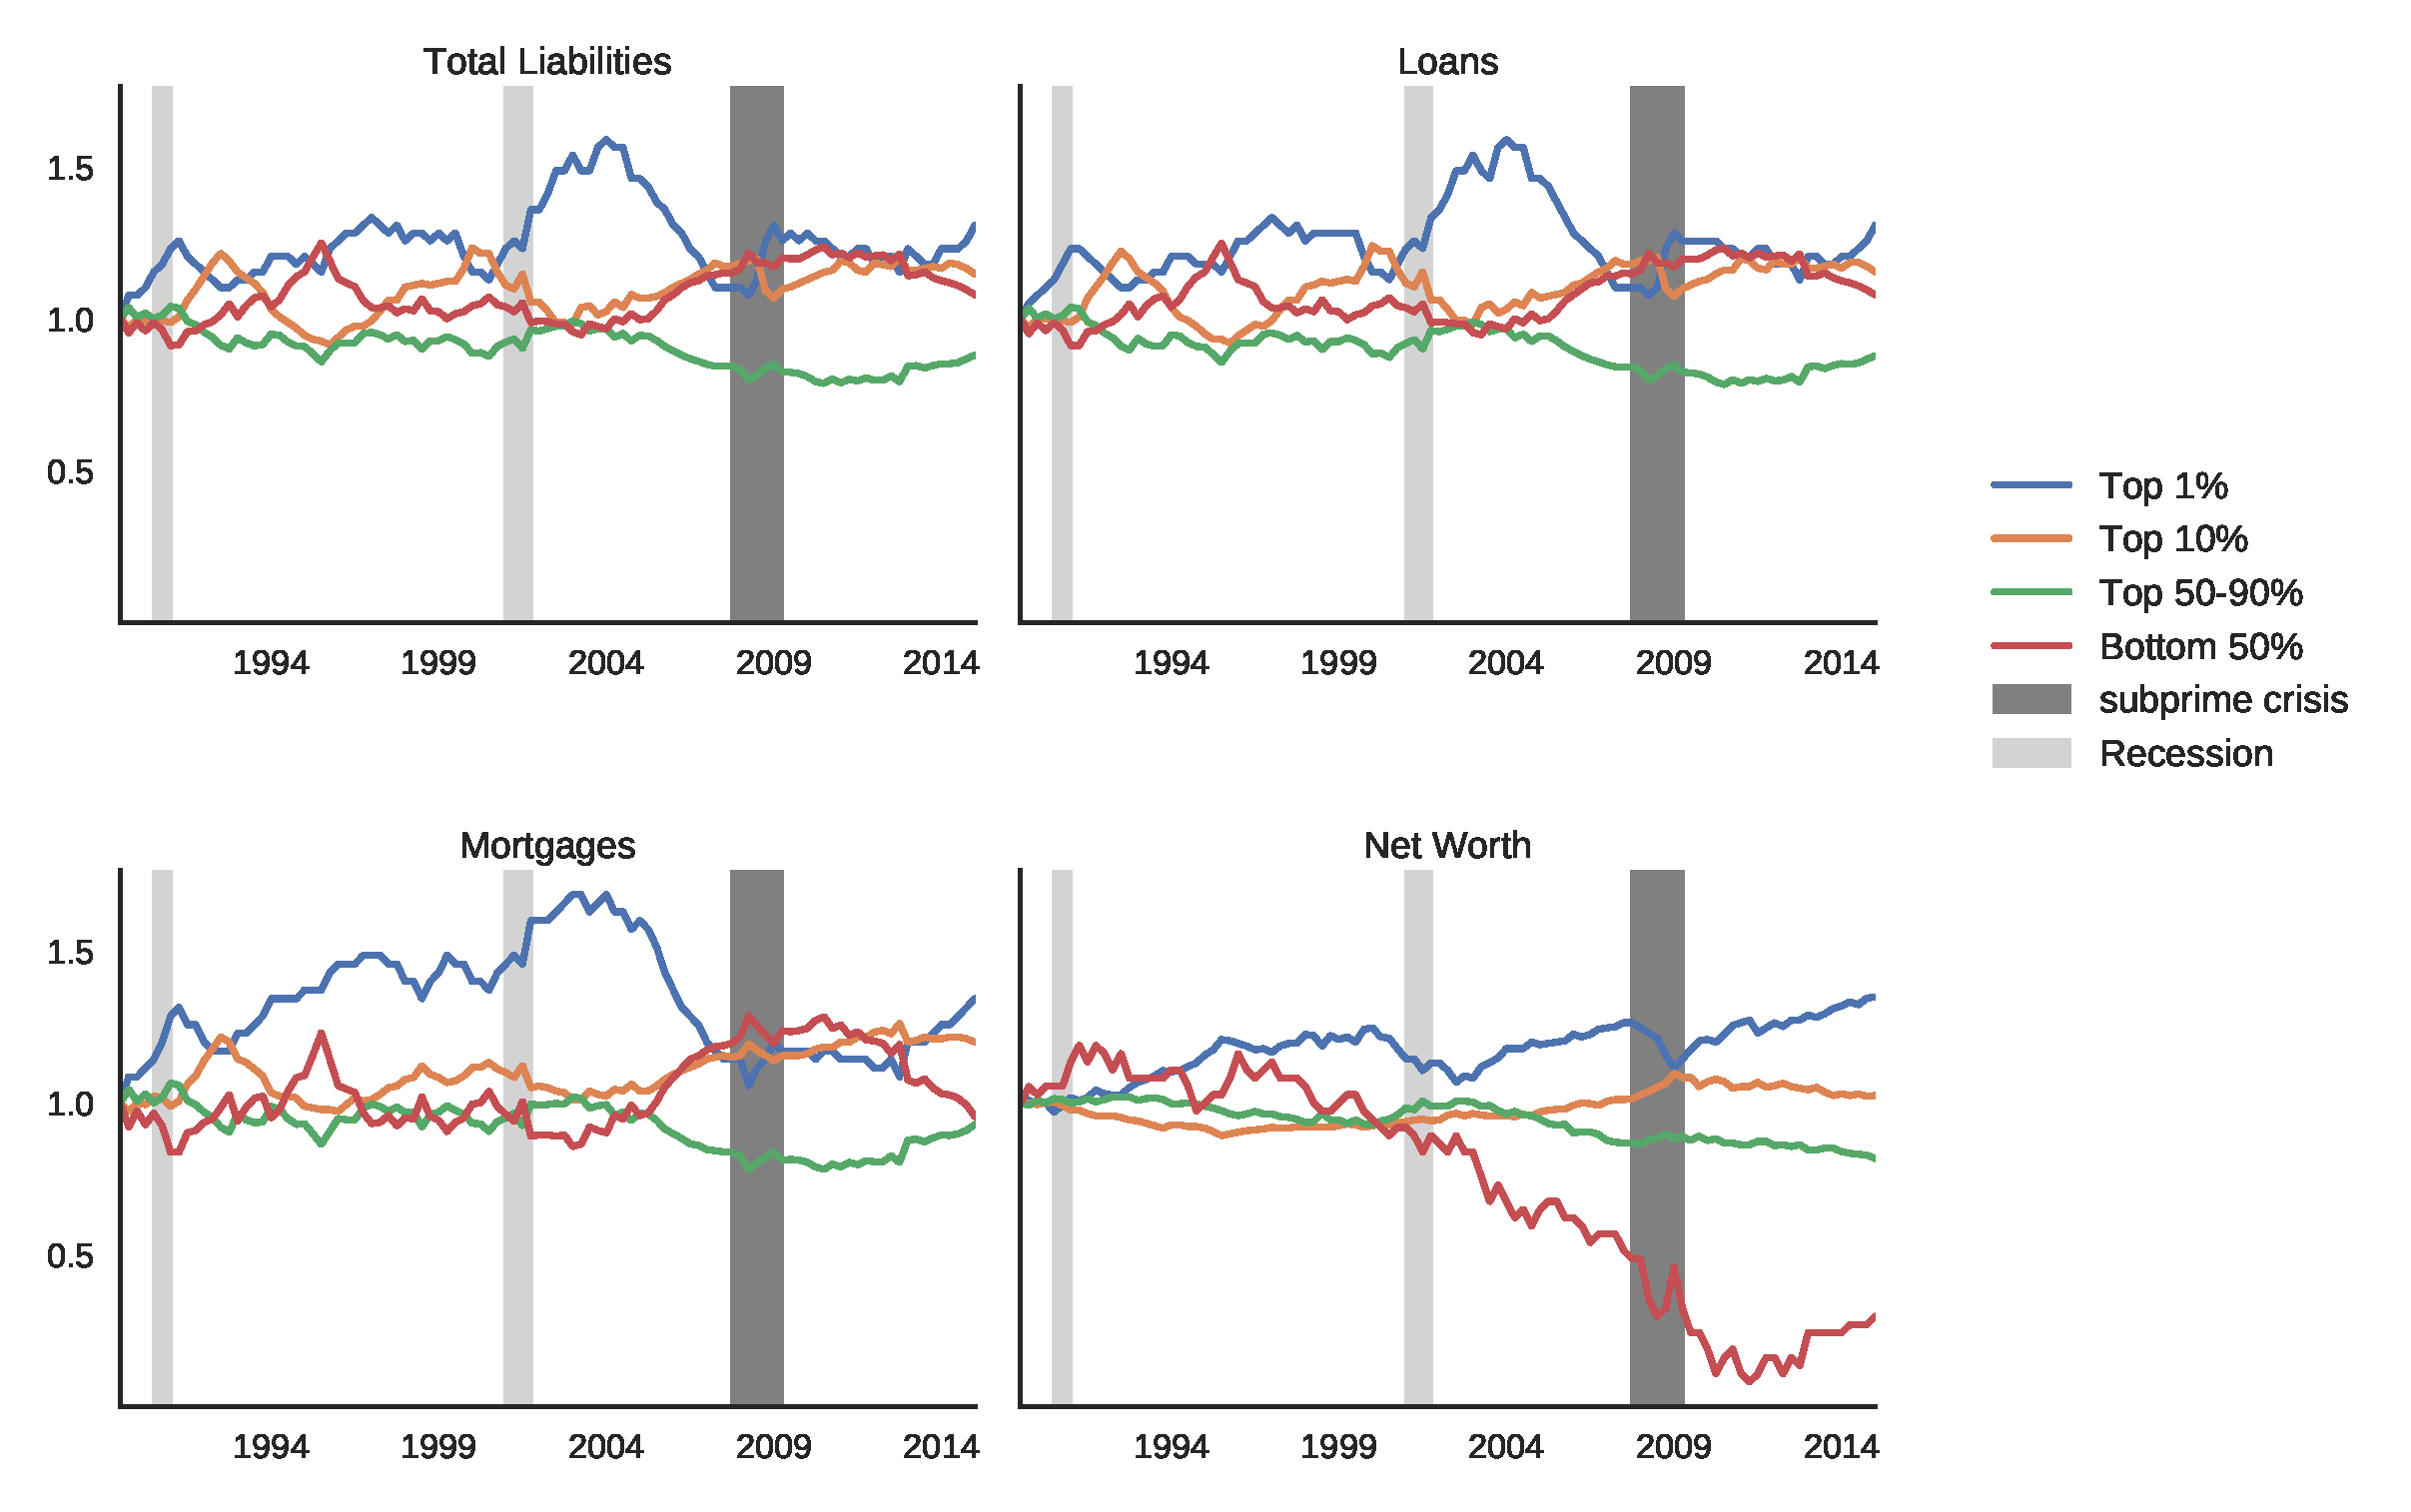
\includegraphics[width=.8\textwidth]{./figs/Distribuicao_Passivos.eps}
	\caption*{\textbf{Source:} \textcite{us_census_bureau_characteristics_2017}, Authors' Elaboration}
\end{figure}

In summary, we conclude that housing is relevant to understand the specificity of US business cycle.
On the following section, we analyze how econometric literature has dealt with the topic.
More precisely, we evaluate macroeconometric works according to its compatibility with Sraffian supermultiplier growth model.
